% Tutamen: A Second-Generation Secret Storage as a Service Platform
% Paper
%
% 2016
%
% Andy Sayler
% Taylor Andrews
% Matt Monaco
% Dirk Grunwald

% SoCC Template: do not change these values
\documentclass[10pt,twocolumn]{article}
\usepackage{times}
\baselineskip 12pt
\textheight 9in
\textwidth 6.5in
\oddsidemargin 0in
\topmargin 0in
\headheight 0in
\headsep 0in

% System Packages
\usepackage{epsfig}
\usepackage{float}
\usepackage{caption}
\usepackage{subcaption}
\usepackage{tabu}
\usepackage{color}
\usepackage{hyperref}
\usepackage{url}
\usepackage{listings}
\usepackage{authblk}

% Package Options
\hypersetup{
    colorlinks,
    citecolor=black,
    filecolor=black,
    linkcolor=black,
    urlcolor=black
}

% Macros
\newenvironment{packed_enum}{
\begin{enumerate}
  \setlength{\itemsep}{1pt}
  \setlength{\parskip}{0pt}
  \setlength{\parsep}{0pt}
}{\end{enumerate}}

\newenvironment{packed_item}{
\begin{itemize}
  \setlength{\itemsep}{1pt}
  \setlength{\parskip}{0pt}
  \setlength{\parsep}{0pt}
}{\end{itemize}}

\newenvironment{packed_desc}{
\begin{description}
  \setlength{\itemsep}{1pt}
  \setlength{\parskip}{0pt}
  \setlength{\parsep}{0pt}
}{\end{description}}


% Other Options
\clubpenalty = 10000
\widowpenalty = 10000

% Start
\begin{document}

%make title bold and 14 pt font (Latex default is non-bold, 16 pt)
\title{Tutamen: A Next-Generation Secret-Storage Platform}

% start author
\author{Andy Sayler}
\author{Taylor Andrews}
\author{Matt Monaco}
\author{Dirk Grunwald}
\affil{University of Colorado}
% end author

%don't want date printed
\date{}

\maketitle

\begin{abstract}
The storage and management of secrets (encryption keys, passwords,
etc) are significant open problems in the age of ephemeral,
cloud-based computing infrastructure. How do we store and control
access to the secrets necessary to configure and operate a range of
modern technologies without sacrificing security and privacy
requirements or significantly curtailing the desirable capabilities of
our systems? To answer this question, we propose Tutamen: a
next-generation secret-storage service. Tutamen offers a number of
desirable properties not present in existing secret-storage
solutions. These include the ability to operate across administrative
domain boundaries and atop minimally trusted infrastructure. Tutamen
also supports access control based on contextual, multi-factor, and
alternate-band authentication parameters. These properties have
allowed us to leverage Tutamen to support a variety of use cases not
easily realizable using existing systems, including supporting
full-disk encryption on headless servers and providing fully-featured
client-side encryption for cloud-based file-storage services. In this
paper, we present an overview of secret-storage challenge, Tutamen's
design and architecture, the implementation of our Tutamen prototype,
and several of the applications we have built atop Tutamen. We
conclude that Tutamen effectively eases the secret-storage burden and
allows developers and systems administrators to achieve previously
unattainable security-oriented goals while still supporting a wide
range of feature-oriented requirements.
\end{abstract}

\section{Introduction}
\label{sec:intro}

How best to store and manage secrets -- the bits of tightly controlled
data necessary to ensure or bootstrap the security of computing
systems and services -- has always been a non-trivial problem. As we
continue to move toward computing and storage platforms controlled by
third parties, and embrace modern trends toward ephemeral
infrastructure, the secret storage problem only becomes more prevalent
and critical to solve.

Tutamen\footnote{Latin -- A means of protection or defense.} is our
attempt to solve the secret storage problem in a manner that allows
the user to adhere to a range of security and privacy requirements
without sacrificing functionality in the process. Tutamen is a next
generation secret storage platform. It builds on our previous secret
storage efforts~\cite{custos-trios} and strives to offer features not
provided by the various secret storage systems available today. In
this paper, we offer several contributions:

\begin{packed_item}
\item The design, implementation, and evaluation of a secret storage
  system with support for several novel features including:
  \begin{packed_item}
  \item Modular authentication modules designed to add use-case
    flexibility through the use of contextual, multi-factor, and
    alternate-band (e.g. SMS text messages) authentication mechanisms.
  \item The ability to operate atop minimally trusted infrastructure
    by leveraging multiple storage and access control providers to
    achieve both redundancy and to mitigate trust.
  \end{packed_item}
\item Several practical demonstrations of how a secret storage system
  with such features can be integrated with real-world applications to
  offer desirable features in a secure and easy-to-use manner.
\end{packed_item}

\subsection{The Need for Secret Storage}

Computing systems today invade every contour of our lives -- from the
fitness trackers on our wrists, to our ``smart'' home appliances, to
the server infrastructure required to support the range of web sites
and services we interact with every day. With this explosion of
computing systems has come an equally large explosion in the amount of
data stored by and about us. While some of this data is designed to be
public (i.e. the entries on Wikipedia), much of it is not, requiring
the enforcement of various privacy and security guarantees with
respect to its handling and storage. The basis of providing such
guarantees relies on our ability to store and selectively share
secrets ranging from the keys used to encrypt our data to the
passwords used to protect our online accounts. How best to store and
manage these secrets is thus a critical question -- the answer to
which forms the foundation to all of computing's higher level security
and privacy guarantees.

Beyond the need to bootstrap a variety of security guarantees, there
are several other factors driving the need for robust secrete storage
solutions. On the system administration front, the trend toward
ephemeral infrastructure cable of rapidly scaling up or down is
driving the adoption of configuration management systems such as
puppet~\cite{puppet} or chef~\cite{chef}. Such systems, however, do
not tend to have suitable mechanisms for enforcing the security and
privacy requirements inherent to storing secrets. Despite this,
configuration data often contains a variety of secrets such as SSH
keys, TLS/SSL keys, file encryption keys, and the tokens or
credentials necessary to authenticate to external APIs and services.

Similarly, on the end-user front, the need for suitable secret storage
systems is being driven by a rapid expansion of the number of sites
and services to which users must authenticate themselves, as well as
by the growing expanse of digital data users wish to protect. Indeed,
the popularity of password management systems such as
LastPass~\cite{lastpass} or 1Password~\cite{onepassword} as well as
user demands for encryption support on their
devices~\cite{intercept-cookencryption} demonstrate the importance of
secret storage, and the applications it enables, to end users.

\subsection{The Ideal Secret Storage System}

Unlike standard configuration management systems, or even specific
secret storage systems such as password managers, a general purpose
secret storage presents a number of unique requirements including the
following capabilities:

\begin{packed_item}
\item Store a wide-range of arbitrary secret data
\item Store secret data in a secure manner
\item Enforce fine-grained access control requirements
\item Support a range of authentication sources/methods
\item Provide audit logs tracking secret access history
\end{packed_item}

In response to these needs, a number of general purpose secret-storage
systems have been recently developed by industry, including
HashiCorp's Vault~\cite{vault}, Lyft's Confidant~\cite{confidant}, and
Square's Keywhiz~\cite{keywhiz}. These systems exist to fulfill some
or all of the requirements listed above. We believe, however, that
such systems are hindered by several key limitations. First, they
generally require at least one fully trusted server as the basis of
their security model, making them unsuitable for operation atop
untrusted infrastructure. Second, they tend to lack support for use
cases requiring autonomous or remote access to secret material in a
secure manner. These deficiencies give rise to a few more secret
storage requirements:

\begin{packed_item}
\item Avoidance of the need to place a high degree of trust in any
  single system outside the application that wishes to store a secret.
\item Ability to support a range of secret access use-cases, including
  use cases where automatic or remote access to secrets is required.
\end{packed_item}

It is toward these final two requirements that Tutamen attempts to
advance the state of the art over existing secret storage systems. In
particular, Tutamen supports operational modes where no single entity
other than the application must be trusted. This allows users to
leverage third party secret storage providers running Tutamen servers
without having to place high degrees of trust in any single
provider. Tutamen also provides support for a modular authentication
interface. This interface makes Tutamen suitable for use in situations
where it is desirable to leverage external environmental information
to automatically evaluate the authenticity of a secret request are
where it is necessary to keep a human in the authentication loop
without actually requiring that the human be physically present or
connected to the application requesting a secret. For example, Tutamen
can be used to store the disk encryption keys required to boot a
headless server, and only release these keys to the server requesting
them when a human responds to a text message confirming the boot
request.

%%  LocalWords:  Tutamen LastPass HashiCorp's Lyft's Keywhiz OOB SMS

\section{The Tutamen Platform}
\label{sec:tutamen}

\subsection{Architecture}

The Tutamen Secret Storage platform has three main components:

\begin{packed_desc}
\item[Access Control Servers (ACS):] The systems responsible for
  storing and enforcing secret access control requirements and for
  authenticating clients making requests.
\item[Storage Servers (SS):] The systems responsible for storing
  secrets (or parts of secrets).
\item[Tutamen Applications (TA):] The systems leveraging the Tutamen
  platform to store and retrieve secrets.
\end{packed_desc}

In general, Tutamen communication occurs between applications and both
types of servers. Tutamen servers do not generally communicates with
each other directly -- with the one exception of storage servers
needing to download the public signing keys from each of the access
control servers with which they interact. All communication in Tutamen
takes place via HTTPS connections - and in some cases leverage mutual
TLS to require both client and server authentication.

Both access control and storage servers are designed to be used
individually or in sets. E.g. An applications may store their secret
on a single storage server and delegate access control to a single
access control server, or the applications may shard its secret across
multiple storage servers and delegate access control to multiple
access control servers, or any combination thereof. By separating the
access control duties from the secret storage duties, Tutamen offers
the end-user a high degree of flexibility to implement a range of
redundancy and trust requirements.

\subsubsection{Access Control Servers}

The Tutamen Access Control Servers are responsible with authenticating
Tutamen requests as well as storing and enforcing all access control
requirements. Access Control servers expose a number of core data
structures that reflect that manner in which they
operate. Figure~\ref{fig:tutamen:acstructs} shows these structures.

\begin{figure}[th]
  \centering
  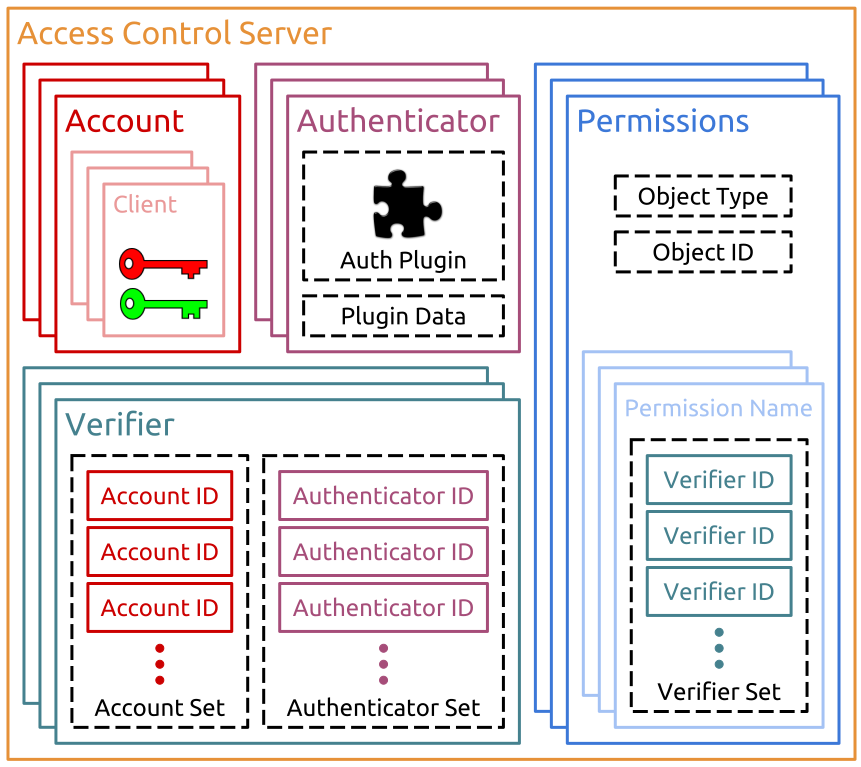
\includegraphics[width=\columnwidth]{./figs/pdf/tutamen-datastructures-ac.pdf}
  \caption{Access Control Server Data Structures}
  \label{fig:tutamen:acstructs}
\end{figure}

In order to track and control access from specific users - the ACS
uses per-user accounts. These accounts are generally designed to to
mapped to individual end-user, but they can be used to track any
singular entity to which one wishes to assign specific access control
privileges. Accounts thus form the basis of controlling and sharing
access to secretes via Tutamen. Within each account are one or more
clients. While accounts map to logically singular access control
entities, clients map to specific devices that will need to make
Tutamen requests. Each account has one or more clients. For example,
Jane Coworker would have a single account with one client for her
laptop, one for her desktop, and one for her phone.

Each client is associated with a single TLS key-pair used to
authenticate the client to the access control server. The access
control server doubles as the Certificate Authority administering
these certificates. When a new client is created it generates a local
RSA key and uses this key to generate an X509 Certificate Signing
Request~\cite{rfc5280}. This request is then sent to the access
control server where it awaits approval from an existing client in the
account. If approved, the CSR is used to generate a signed certificate
that is sent back to the new client for use in future access control
server communication. To facilitate bootstrapping new account, clients
keys and CSRs are also generated and sent with each new account
request. These are atomically approved and associated with the new
account -- i.e. the initial client is created in tandem with a new
account -- all subsequent clients are then approved by previously
approved clients.

While accounts and clients are used to identify specific
users/entities -- the Tutamen access control server also has
authenticators. Authenticators are modular mechanism used to implement
access control requirements beyond granting access on the basis of
accounts. For example, authenticators can support plugins to perform
additional contextual authentication requirements such as only
allowing access during specific times of day, or from requests
originating form specific IP addresses. Authenticators can also be
used to implement out-of-band authenticators mechanism such as
requesting approval for a specific request from a user via text
message or otherwise interfacing with eternal services to gain
approval.

Accounts and authenticators are combined via verifiers. A verifier
consist of a set of Accounts and a set of Authenticators. In order to
satisfy a verifier a request must originate form ONE of the Accounts
and must satisfy ALL of the authenticators plugins listed in the
verifier. A verifier may contain no Authenticators, in which case
authorization is granted solely on the basis of accounts.

The final component of the Tutamen access control specification are
permission groups. Each permission group corresponds to a specific
object (identified via the combination of an object type and an object
ID) within the Tutamen ecosystem. A permission groups contains one or
more permissions - each corresponding to a specific class of actions
that can be preformed on the corresponding object. Each permission
contains a set of verifiers. In order to be granted a given permission
a request must satisfy at least one of the verifiers in this set.

\subsection{Security and Trust}

\subsection{Implementation}

%%  LocalWords:  Tutamen ACS HTTPS CSR CSRs Authenticators verifiers
%%  LocalWords:  authenticators

\section{Security and Trust}
\label{sec:trust}

One of Tutamen's primary design goals is its ability to support a wide
range of security and trust requirements. It achieves this goal
through its support for both centralized and distributed operation as
well as though its support for a range of authentication mechanisms.

\subsection{Security of Individual Servers}

The security of each individual access control server rests on several
requirements. Failure to uphold these requirements will result in the
failure of any security guarantees provided by the AC server.

\begin{packed_desc}
\item[Certificate Authority Role:] Each access control server acts as
  a CA delegated with issuing and verifying client certificates. Thus,
  each AC server must store its CA keys in a secure manner and
  faithfully verify the certificate presented by each client
  connection.
\item[Token Issuance and Verification:] Each access control server is
  responsible for verifying the access control requirements bound to
  specific object/permission combinations, issuing signed tokens
  attesting to such verification, and verifying the signatures of the
  tokens it receives from clients wishing to operate on access control
  objects. Thus, each AC server must store private token signing key
  in a secure manner and faithfully verify both the access control
  requirements governing specific token requests as well as the
  signatures on all incoming tokens.
\end{packed_desc}

The storage servers must uphold the following security
requirements. Failure to do so results in a failure of the security of
the storage server.

\begin{packed_desc}
\item[Token Verification:] Each storage server must securely (via
  HTTPS) obtain the public token signing key from each AC server
  delegated with providing access control for a given storage
  object. The storage server must then use these keys to faithfully
  verify the signatures on all tokens it receives. Assuming the token
  signature is valid, the storage server must faithfully enforce the
  claims asserted in a given token; e.g., by only allowing actions
  granted by the permission contained in the token on the object the
  token identifies prior to the expiration time specified by the
  token.
\item[Secure Storage:] Each storage server must take steps to store
  user-provided secrets in a secure manner, releasing them only to
  requests accompanied by the requisite number of valid tokens
  granting such release.
\end{packed_desc}

Since the tokens the storage server must verify are provided by the AC
servers, the security of the storage server with respect to a given
collection is dependent on the security of any designated AC servers
associated with said collection. If these AC servers are insecure, the
objects that delegate access to them will also be insecure.

\subsection{Security of Multiple Servers}

Unlike existing secret management systems~\cite{vault, confidant,
  keywhiz}, the Tutamen architecture is capable of remaining secure
even when individual storage or access control servers fail to meet
their security requirements. Such failures may result from physical
server compromise, software bugs, malicious intent or incompetence on
the part of the server operator, or compelled failures.\footnote{For
  example, being forced to turn over stored secrets in response to
  legal or governmental pressure.}

To work around security failures of individual server, Tutamen
applications can leverage Tutamen's distributed operation modes. In
these modes, the security of the system as a whole is diffused, no
longer relying on the security of any specific access control or
storage server in order to keep an application's secrets secure. As
described in Section~\ref{sec:tutamen:arch:distributed}, each
application can distribute both secret storage and access control
delegations using $n$ choose $k$ schemes. In such setups, the
difference between $n$ and $k$ represents the degree to which a
Tutamen applications can withstand security failures of the associated
AC and storage servers. For example, an application which chooses to
shard its secrets across five storage servers where any three shards
are sufficient to recreate the secret ($n=5$, $k=3$) will continue to
remain secure even if two of the storage servers fail to meet their
security obligations. Similarly, if each secret shard delegates five
possible AC servers, tokens from three of which are required to grant
secret access, the applications can withstand the failure of two AC
servers to uphold their security guarantees.

\subsection{Trust Model}

Trust in Tutamen follows from the security models of both individual
Tutamen servers and of the distributed Tutamen deployment
architectures. If a Tutamen application is leveraging only a single
storage and AC server, the application is placing a high degree of
trust in both servers (and by proxy, the operators of both
servers). This level of trust may be appropriate for some use cases
(e.g., when a user is operating their own Tutamen's servers), but is
inappropriate in many other cases (e.g., when using third party hosted
Tutamen servers). Fortunately, Tutamen allows applications to avoid
placing a high degree of trust in any single server by leveraging
multiple servers and picking $k$ and $n$ in a manner commensurate with
the degree to which each server is trusted.

Beyond minimizing the amount of trust placed in each individual
Tutamen server by leveraging multiple servers, we also envision
economic incentives helping to ensure Tutamen server
trustworthiness~\cite{anderson2001}. The Tutamen protocol is
standardized and designed to support a range of interchangeable ACS
and SS providers. Such a design allows for the development of a
Tutamen server marketplace where both ACS and SS providers can compete
against each other on the basis of trustworthiness, features (e.g.,
what types of authenticators they support), and cost. In such an
ecosystem, Tutamen service providers who fail to uphold the Tutamen
security requirements on their servers will suffer a negative economic
effect, disincentivizing such behavior. It is also likely that storage
providers who take additional steps to protect the secrets they store
(e.g., by using systems such as Trusted Platform Modules (TPMs) to
encrypt the secrets they hold and harden server security) would be
able to command a higher price in the marketplace, incentivizing such
best practices.

Thus, unlike other third-party cloud services where trustworthiness
and economic incentives are in direct competition (as is the case on
many ``free'' third part services that depend on selling user data in
order to generate revenue)~\cite{flowerday2006}, Tutamen encourages a
system where economic incentives are well aligned with user
trust. That fact, coupled with the high degree of control over
third-party trust Tutamen grants to each application by allowing each
application to select how many servers to diffuse trust across, make
Tutamen a robust system in the face of both security and
trustworthiness failures. Such robustness is a critical component of
any successful secrete storage system.

%%  LocalWords:  Tutamen's Tutamen CAs DNS TPMs authenticators HTTPS
%%  LocalWords:  ACS

\section{Example Applications}
\label{sec:apps}

Tutamen is designed to support a wide range of applications. We have
integrated our reference Tutamen design with a set of common
applications for the purpose of demonstrating the value derived from
using a secure storage system such as Tutamen. These applications all
leverage Tutamen's flexibility to achieve functionality that would
have been difficult or impossible to achieve without using a system
like Tutamen.

\subsection{Block Device Encryption}

Block device encryption systems are a popular means of protecting the
data stored on computing systems in the event that the system is lost,
stolen, or otherwise physically compromised.  Block-level encryption
systems such as dm-crypt~\cite{dm-crypt} (generally coupled with the
Linux Unified Key Setup (LUKS)~\cite{luks} container) or the
QEMU~\cite{qemu} qcow2 encryption system provide methods for securing
the data stored on laptops, desktops, and VMs. Such systems
traditionally bootstrap security by requiring the user to enter a
password at boot-time to unlock a locally stored encryption key which
is then used to decrypt the block device in question. Unfortunately,
the ``human-at-the-keyboard'' security root make such systems
difficult or impossible to use atop headless servers or in situations
where no human can be expected to be present at boot-time. We have
leveraged Tutamen to overcome this barrier.

To add Tutamen-support to LUKS/dm-crypt we have integrated Tutamen
with the LUKS/dm-crypt bootstrapping
process~\cite{src-tutamen-askpassword}. Our integration replaces the
traditional ``human-at-the-keyboard'' boot-time password prompt with a
request to a Tutamen storage server for necessary decryption secret
(after first retrieving the necessary tokens from the corresponding
Tutamen AC server). We have also integrated Tutamen support with QEMU
to provide qcow2 encryption keys when a VM
boots~\cite{src-qemu-tutamen}. Similar to the dm-crypt setup, QEMU
normally requires the user to provide the encryption key via the QEMU
console when a VM launches. Our system replaces this process with
Tutamen-based secret retrieval. Using these setups, we're able to boot
servers and VM images with encrypted disks without requiring a human
to be physically present at the machine. In cases where we still
desire human approval of the boot process, we can leverage our SMS
authenticator module to get an on-demand confirmation from a
designated human as a prerequisite to Tutamen releasing the correct
key. This allows us to gain the same level of human-in-the-loop
security provided by a typed passphrase, but without actually
requiring a human to go to the datacenter to type one in. In
situations where we don't desire a human-in-the-loop at all, we
envision automating the approval process via the use of time-of-day
and IP-source authenticators.

\subsection{Encrypted Cloud Storage}

Cloud-based file storage systems such as Dropbox~\cite{dropbox} are
extremely popular today. Unfortunately, these systems require users to
trust the cloud provider with full access to their (generally
unencrypted) data. Users wishing to overcome this deficiency can
optionally encrypt all of their data on the client before syncing it
to the file locker provider, but doing so does not generally interact
well with such services' sharing and multi-device use cases, requiring
users to employ manual, out-of-band key exchange mechanisms to share
or sync their encrypted files. We don't believe file locker users
should have to choose between easily syncing or sharing their files
and using encryption to protect their data. Tutamen provides a
solution to this problem by offering a secure key-sharing
mechanism. Instead of manually distributing or sharing encryption
keys, the user can store their key as a Tutamen secret and leverage
Tutamen's access control features to share the secret with the
accounts of their friends. This entire process can even be automated
such that when a user shares a file via Dropbox, the corresponding
encryption key is automatically shared via Tutamen.

Toward this end, we have created FuseBox~\cite{fusebox}: an alternate
Dropbox client that performs client-side encryption of all Dropbox
files, storing the corresponding encryption keys on our reference
Tutamen server. FuseBox achieves goals similar to those achieved
by~\cite{goh2003}, but without requiring out-of-band key
management. Similar to other file-system-level encryption
systems~\cite{blaze1993, Cattaneo2001, halcrow}, FuseBox provides
transparent file encryption to end users. In order to avoid the
storage space and security challenges presented by locally caching all
Dropbox data (i.e., the operation mode for the official Dropbox
client), FuseBox uses AES~\cite{daemen1999, nist2001} as a stream
cipher to transparently stream and encrypted data to/from Dropbox's
servers on demand. Since FuseBox leverages Tutamen to store each
per-file encryption key, FuseBox natively supports Dropbox's
multi-device sync use case by allowing a user to access and decrypt
their Dropbox files from any device on which they have setup the
Tutamen client. FuseBox also makes it simple to share an encrypted
file via Dropbox, share its encryption key via Tutamen, and achieve
the same level of functionality traditional Dropbox users have without
having to expose one's data to Dropbox.\footnote{While the key sharing
  process in FuseBox is not yet directly synced with Dropbox's file
  sharing system, the Tutamen CLI can be used to quickly share the
  encryption keys between users.} In this manner, we have used FuseBox
to store and share encrypted files with nearly the same ease with
which one might use the traditional unencrypted Dropbox client. By
leveraging Tutamen, FuseBox also gains the ability to remotely revoke
file access, e.g., in the case a device is lost or stolen, similar to
systems such as~\cite{geambasu2011}. FuseBox, via Tutamen's
distributed operation mode, also avoids the sharing pitfalls
associated many existing ``secure cloud storage''
providers~\cite{wilson2014} by avoiding reliance on a single trusted
party to facilitate sharing operations.

%%  LocalWords:  Tutamen keyslots keyslot systemd cryptsetup initrd
%%  LocalWords:  libcryptsetup initramfs Archlinux RedHat ini pid FDE
%%  LocalWords:  dgram tutamen OpenVPN TUTATEM luks authenticators dm
%%  LocalWords:  SMS authenticator golang Tutamen's FuseBox FuseBox's
%%  LocalWords:  QEMU qcow

\section{Evaluation}
\label{sec:eval}

We've evaluated Tutamen in a variety of scenarios. These scenarios
have proven Tutamen's usefulness as an enabler of previously
unattainable functionally and use cases. While Tutamen is still a
prototype, we feel it provides a well designed architecture capable of
supporting a wide range of practical secret storage applications.

\subsection{Server Performance}

Our Tutamen reference implementation provides a usable prototype with
which to experiment with Tutamen applications. While the server
software has not yet been optimized for performance, we have performed
a number of performance measurements in order to better understand the
computational load a system like Tutamen requires.

\begin{figure}[th]
  \centering
  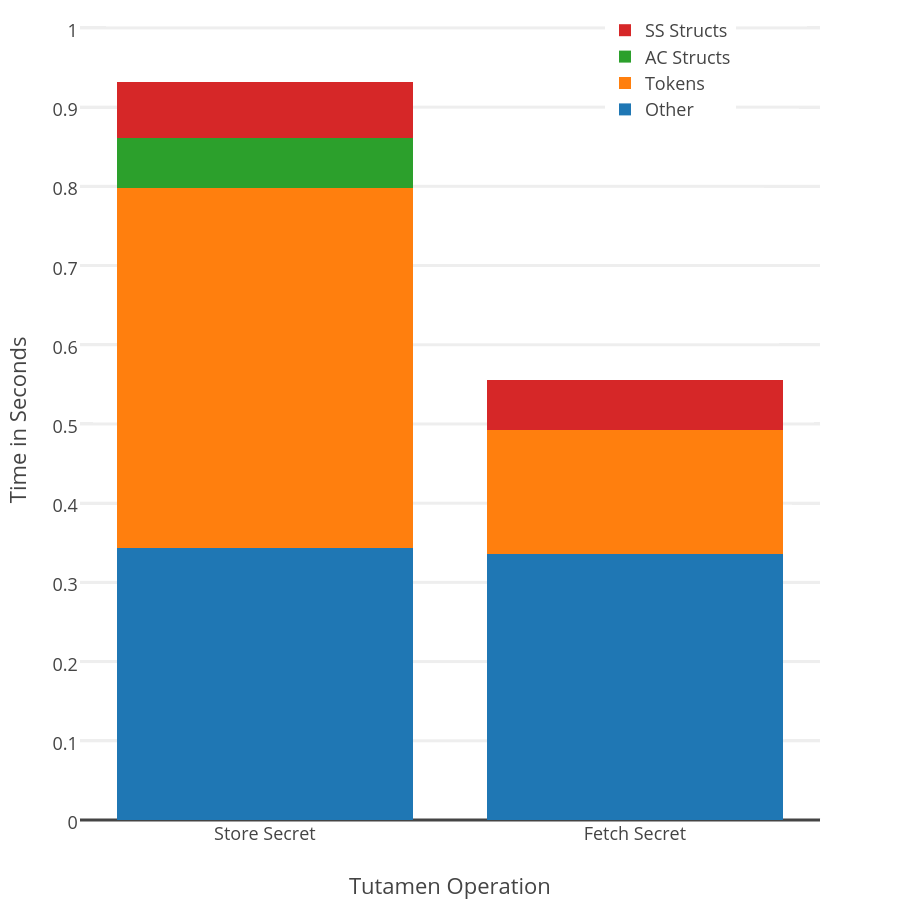
\includegraphics[width=\columnwidth]{./figs/png/chart-combined-timings.png}
  \caption{Timings for Tutamen Operations}
  \label{fig:eval:timings}
\end{figure}

Figure~\ref{fig:eval:timings} shows the time required to complete two
of the most common Tutamen operations: storing a new secret and
retrieving a previously stored secret. We measured the amount to time
the Tutamen CLI application spent performing various parts of each of
these two Tutamen operations. In both operations, the bulk of the
server-related run time is spent requesting and retrieving the
authorization tokens required to complete the associated
operations. In the secret creation case, five tokens are
required\footnote{Two permission group creation tokens (one for the
  collection permission group and one for the verifier itself), one
  verifier creation token, one collection creation token, and one
  secret creation token.}. In the secret read case only a single token
is required\footnote{The collection read permission token}. The
reminder of the server-related time is spent either creating AC and
storage data structures (as in the store secret case) or reading
existing data structures (as in the retrieve secret case). The
``other'' time is spent reading the Tutamen config files, loading the
necessary client certificates, and dealing with the overhead required
to interpret the python-based CLI.

It is not unexpected that the client must spend the bulk of its time
requesting tokens and waiting for them to be approved -- token
verification is the primary role the access control server must
perform, and depending on the complexity of the verifiers associated
with the permission the token is requesting, verification can be a
fairly complex task. When performing these measurements, we employed a
simple verifier that only required client membership in a specific
account. Verifiers that include human-in-the-loop authenticators
(e.g. SMS approval) would increase the token turnaround time by the
amount of time the human requires to provide approval. Thus, it's
important that Tutamen applications treat token approval as an
operation that can take anywhere from under a second to 10s of
seconds. To help alleviate these waits on applications that must
perform a high number of Tutamen requests, our deign allows Tutamen
tokens to be reused up until their expiration time. Thus, its possible
for an applications to request a long lived token\footnote{Token
  expiration time is included in data presented to each authenticator
  module -- it's thus possible for these modules to factor the token
  length into their decisions regrading whether or not to approve the
  token request. This is useful in cases where a module wishes to
  require a higher level of confidence in the validity of a request
  for long-lived tokens.} and to reuse this same token to access
e.g. multiple secrets within the collection to which the token grants
read access.
 
\begin{figure}[th]
  \centering
  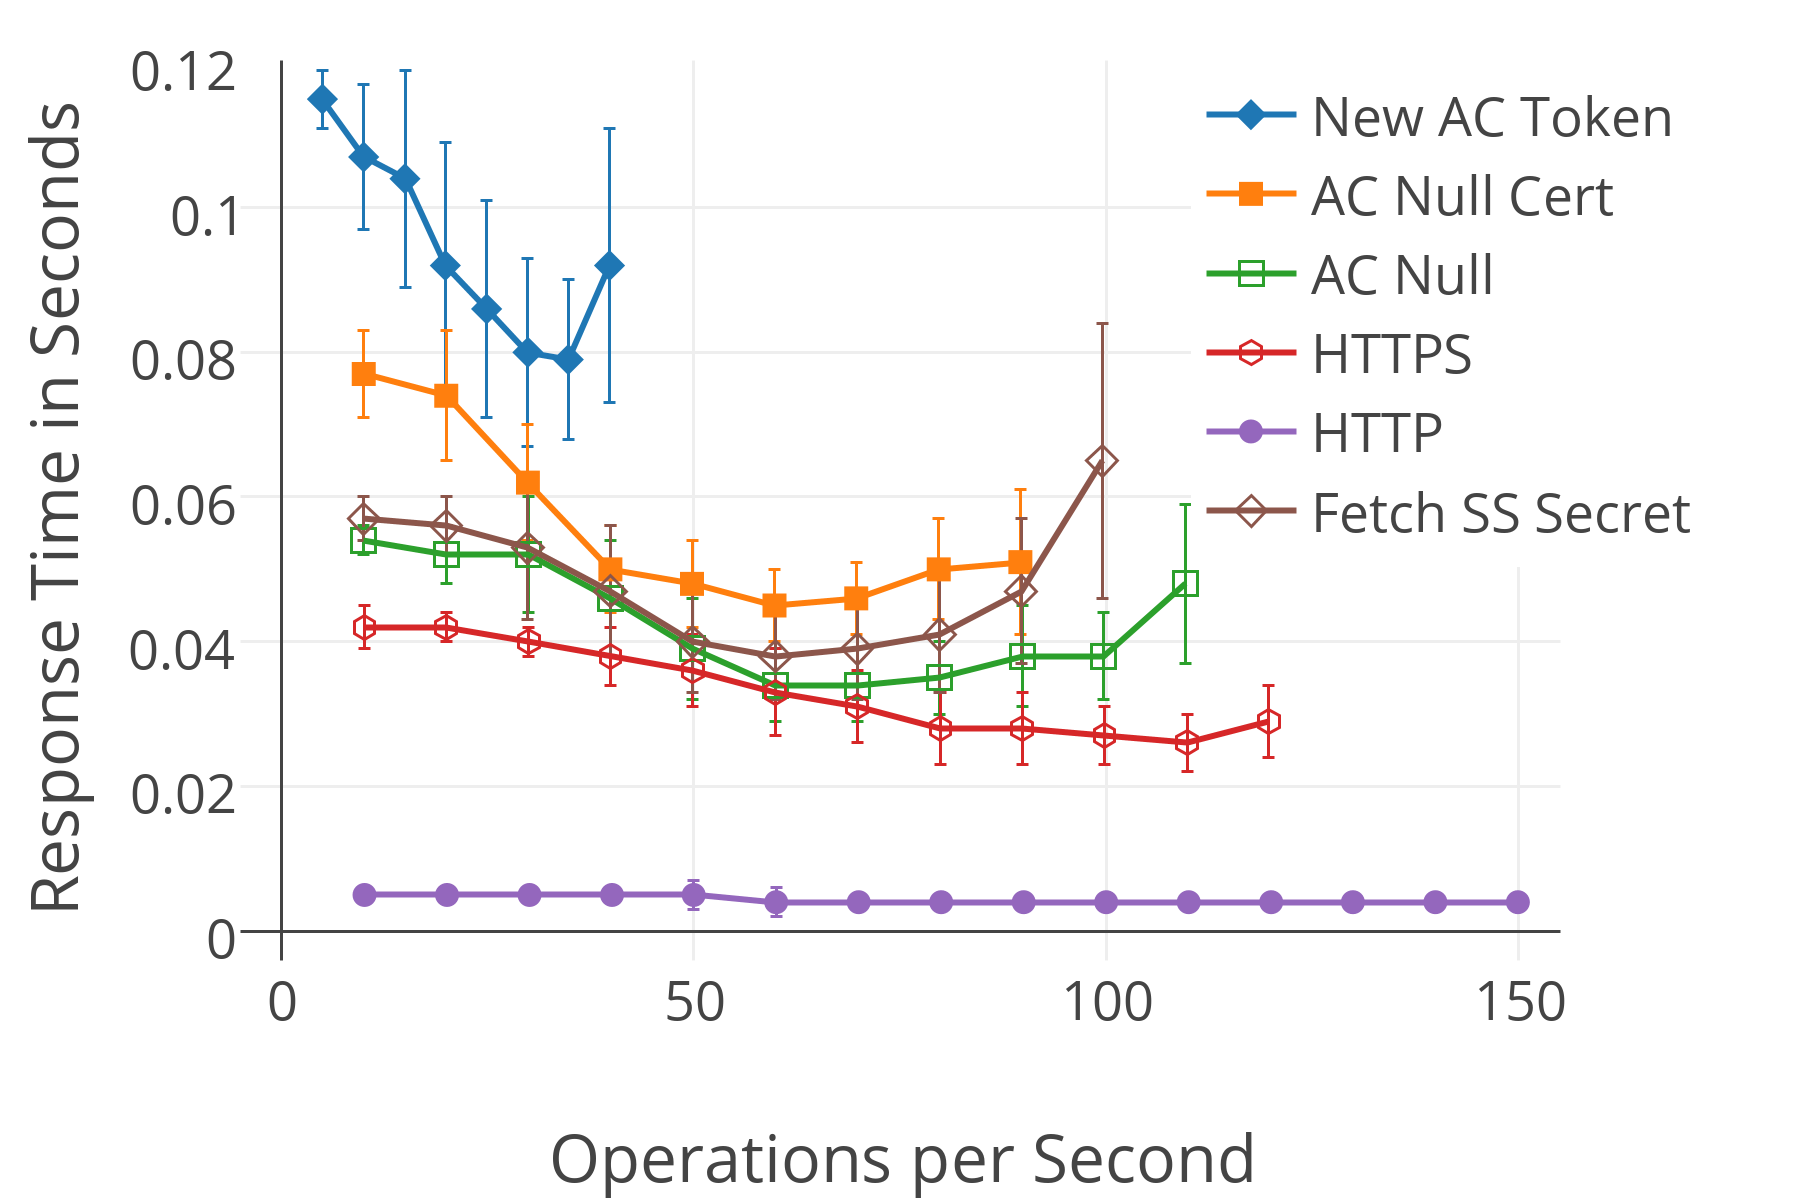
\includegraphics[width=\columnwidth]{./figs/png/chart-iops.png}
  \caption{Throughput vs Latency}
  \label{fig:eval:iops}
\end{figure}

Figure~\ref{fig:eval:iops} shows the request rate vs response time
(with standard deviations) of a single access control server for both
the token request operation as well as for two ``null'' operations:
one which loads a simple ``Hello'' message (but that still verifies
the client TLS certificate required to perform most Tutamen AC server
operations) and one which loads the same message but without providing
or verifying client certificates. As these curves show, token
verification of our prototype server tops out at around 40
requests/second on moderate hardware (e.g. a 4-core, 4GB VM running
atop 2011-era Intel Xeon hardware). The null operation with client
certificates top out around 60 requests per second and the null
operation itself tops out at about 70 request per second. The current
server setup is thus primarily limited by the TLS and WSGI overhead
required to serve the application. Token verification itself does
ensure additional computational requirements - largely limited by the
database speed required to provide access to all of the necessary data
structures that must be inspected in order to evaluate the validity of
a given token request.

% Todo: Storage server curves?

While these levels of performance would not likely meet the
requirements of a production-level Tutamen AC server, they have been
perfect adequate for our needs and have been cable of supporting the
handful of Tutamen applications we're currently using. Since must of
our Tutamen applications require only a single Tutamen secret
retrieval at relatively rare rates (e.g. once per server reboot, or
once per file open) the 30-40 requests per second or server can
provide have been more than adequate for our needs. We've also
designed our reference server to be horizontally scalable in both its
HTTPS request handling (e.g. by spinning up multiple load-balanced
front-end servers each ruining their own Apache WSGI instance) as well
as in its backing database (Redis is capable of distribution across
multiple systems). That scalability, couple with future
performance-related code optimization lead us to believe the Tutamen
server infrastructure can be adopted to meet the needs of larger
installations with only moderate effort.

\subsection{Usage}


%%  LocalWords:  Tutamen Tutamen's verifiers authenticators SMS Xeon
%%  LocalWords:  authenticator HTTPS Redis

\section{Conclusion}
\label{sec:conclusion}

How best to securely store secrets is a pressing issue in today's
cloud-oriented, third-party hosted, ephemeral-infrastructure adopting
environment. This need has triggered the creation of several
secret-storage frameworks and systems. Unfortunately, these existing
systems prove deficient in at least three key secret-storage
capabilities: the ability to support operation outside of a single
administrative domain, the ability to operate atop untrusted
infrastructure, and the ability to support a wide range of use cases.

We created Tutamen to demonstrate our concept for a next-generation
secret-storage system. Tutamen supports client-controlled secret
sharding to allow applications to leverage minimally-trusted server
infrastructure. Tutamen also supports a flexible and modular
authentication mechanism that allows end users to specify complex
access control requirements. We've successfully coupled Tutamen with a
number of applications, including full disk encryption on headless
servers and client-side encrypted file sharing between multiple
parties. These use cases would be difficult (or at least burdensome)
to realize without a system such as Tutamen.

We plan to continue developing the Tutamen ecosystem. On the
server-side, we have plans to work toward increased performance and to
add support for additional authenticator modules. While the Tutamen
servers currently have basic logging support, we also plan to expand
this support, and to explore interfacing Tutamen audit logs with
intrusion detection systems in order to expose more actionable
intelligence to Tutamen authenticator modules. We are also considering
tying Tutamen's logging infrastructure to a public audit system
similar to~\cite{laurie2013}. Such a system would help to further
reduce the trust Tutamen users must place in individual Tutamen
servers by exposing mechanisms by which a user could reliably audit
the behavior of such providers.

We have made all of the Tutamen source code available via the
previously referenced repositories. We encourage others to experiment
with our Tutamen prototype and reference implementation, or to
integrate Tutamen with their projects or applications. We hope that
Tutamen (or similar secret-storage systems) can help to ease the
secret-storage burden currently imposed on administrators, developers,
and end users by providing an alternative to manually managing
sensitive secrets in a manner that also minimizes third party trust.

%%  LocalWords:  Tutamen authenticator Tutamen's


{
%  \clearpage
%  \footnotesize
  \bibliographystyle{abbrv}
  \bibliography{refs}
}

\end{document}

%%  LocalWords:  Tutamen Tutamen's
